%---------------------------------------------------------------------------------
\chapter{Evaluation of VAD Techniques}
\label{chp:comparison}
%---------------------------------------------------------------------------------

%The previous chapter has reviewed a wide class of techniques for VAD, many of which has not been tested thoroughly with other state-of-the-art techniques.
Given the numerous approaches proposed for VAD in the literature, it is clear that the evaluation and bench-marking of these algorithms is important.
In many research reviewed in the previous chapter, the proposed VADs have not been tested and compared thoroughly with other state-of-the-art techniques.
Most of these experiments considered VAD as a holistic system, leading to unfair comparisons. For example, some works \cite{} compared VAD systems that include hangover schemes to ones that do not. In \cite{}, pre-processing techniques such as speech enhancement and noise reduction were applied to VAD systems for comparing against ones that perform directly on raw data. The audio corpora used also vary across different research, leading to slightly different results \cite{}.

This chapter fills in the gap of existing works by putting together the existing VAD techniques in a common testing framework for comparison. To enhance fairness, the comparison is divided into two distinct experiments, correspondingly to the two main modules of VAD as reviewed in the previous chapter. The first part compares the features in terms of discriminative power under different noise conditions; and the second part compares the performance of different decision rules, which produces the final VAD output.

\section{Features}
% 1. comparing discriminative power of features:
%   . energy
%   . sub-band energy
%   . MFCC
%   . harmonicity
%   . LTSD
%   . entropy
%   . PAR
%   . LTSV
%   . LRT coefficients <-- how to say that it can also act as features...

% 1.1 comparing distribution of different features
% 1.2 comparing harmonicity-based features on detecting the voiced speech

Existing evaluation systems \cite{} have provided insights into how the evaluation of features for VAD can be performed efficiently. First, it is observed that a large data set is essential for an adequate evaluation. Such a data set can ensure the coverage of different speaker-dependent variability such as age, sex, accent, emotion, etc. Another important fact learned is that noise condition varies across different applications, yet no single theory seems to exist that can cover all cases. This suggests that the evaluation should distinguish the results from the different application settings. For example, there are many features that can maintain considerable discriminative power under most noise types, but fail drastically under babble noise. On the other hand, some features, such as harmonicity-based features, are designed specifically to work under severe babble noise environments. Thus, averaging the performance of these two classes of features over all noise cases would not make much sense.
Details of the evaluation methodology are provided as follow.

\subsubsection{Database}
There are many speech copora existed that has been used for VAD evaluation. The choice of dataset is sometimes dependent on the speaking language of the authors and the nature of the research project they work on. For example, Ramirez \etal tends to use Spanish datasets such as the SpeechDat-Car \cite{moreno2000speechdat}; while Ishizuka \etal prefers the AURORA-2J Japanese dataset \cite{nakamura2005aurora}. For English language, TIMIT \cite{garofolo1993darpa} and AURORA-2 \cite{pearce2000aurora} databases are among the most commonly used. For the evaluation of VAD features, TIMIT is preferred since it provides manual transcription down to word and phoneme-level. This is tremendously helpful when evaluating the distribution of the features, assuming that the manual transcription is of acceptable accuracy. For example, word-level transcription can be used to plot the distribution of speech against non-speech, and phoneme-level transcription for voiced speech against unvoiced speech plus noise.

A quick look at TIMIT manual transcription showed that they were not perfectly labelled. For example, segment (a) in \fig{timit_groundtruth} was labeled with speech, but its energy is closed to be silence. On the other hands, using energy measure cannot determine non-speech segments with breaths. Thus, a combination of both manual label and energy was employed to estimate the ground truth of each speech utterance.

\begin{figure}[hh] 
    \centering
    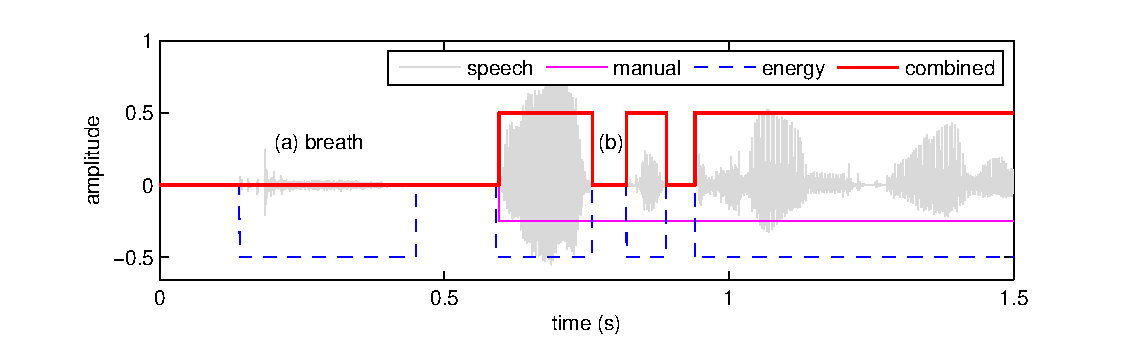
\includegraphics [scale=.8]{timit_groundtruth.eps}
    \caption[Determine referenced VAD labels for TIMIT dataset]{Combining manual labels and energy-based VAD to determine referenced labels for TIMIT utterences. Manual label helps to remove breath regions (a), while energy-based VAD helps to remove very low energy regions (b). (Utterance FECD0/SI788)}
    \label{Fig:timit_groundtruth}
\end{figure}

\subsubsection{Representation}
The evaluation of different features VADs relies on their distribution across the different noise conditions. The separateness of the distributions for speech and non-speech classes represents the discriminative power.

\subsection{Experiment 1: Comparison of features for speech/non-speech classification}

-

-

-

-

- Figure for experiment 1

-

-

-

-

\subsection{Experiment 2: Comparison of features for voiced speech detection}
-

-

-

-

- Figure for experiment 2

-

-

-

-

-

-

-
\subsection{Conclusion}
The performance of various features for VAD was studied in this section. The experiments reveals that...

\section{Decision rules}
% 2. comparing classification power of decision rules:
%   . thresholding
%   . LRT+GMM model
%   . LRT+LD model
%   . LRT+GgammaD model
%   . SVM
%   . MMC
%   . ANN
%   . LDA
%   . PNN
%   . GA

\subsubsection{Database and Features}
Similar to the previous experiments for features evaluation, TIMIT is chosen to evaluate the classification power of different decision rules for VAD. In many evaluation approaches in the literature, the decision rules were compared using different set of features \cite{}. These results did not prove that the marginal discrimination power of a VAD system over one another achieved was due to the feature set used or the actual classifiers employed in the decision rules. The expriment in this subsection compares the different decision rules on the same feature vectors, which shows the relative performance of the classifier used. The experiment is repeated over different set of feature vectors to explore the many configuration posibility.

\subsubsection{Evaluation Metrics}
VAD is a two class classification problem in which there exist trade-offs between the different metrics. Depending on different applications, improvement of one metric might be more desirable, even at a reasonable decrease of the other metric. For example, \emph{precision} and \emph{recall} can be used to measure VAD performance. Precision measures the rate of accurate detection among the detected speech frames, while recall measures the amount of speech frames detected \cite{}. Typically, when the possible parameters of a VAD algorithm is tuned to improve speech detection precision, which implicitly raise its level of strictness to reduce the misdetection, its recall metric  is worsen, and vice versa. This pair of metrics can be used in various application when knowledge of the relative cost of misdetection and incorrect detection is known. For example, for the speech recognition application, it is crucial to have most of the spoken speech frames detected to be able to recognize the whole sentence; while in a speaker diarization and speaker identification, precise detection is preferred to enhance the purity of speaker models. In other applications where the relative cost of speech detection and \emph{non-}speech detection is rather important, the \emph{sensitivity} and \emph{specificity} metric pair is often used. Sensitivity is the same as recall, which measure the true positive detection rate or hit rate, while specificity measure the true negative detection rate. In speech coding applications, sensitivity is used to maximize the amount of speech encoded, while specificity aims to minimize the total bandwidth used.
A common approach to determine the performance for VAD while using these pairs of metrics is via the Receiver Operating Characteristics (ROC) curve, in which one's aim is to maximize the area under the curve (AUC).

TODO: what about Freeman et al, Beritelli et al? (check Ghosh11)
TODO: using Bhatta..yya coefficient to measure overlapness.

\subsection{Experiment 3: Comparison of decision rules for VAD}
-

-

-

-

-

-

- Lots of figures go here

-

-

-

-

-

-

-

-

\subsection{Conclusion}
This section studied and evaluated the different decision rules for VAD proposed in the literature. From the experiments, it is shown that...
%---------------------------------------------------------------------------------%
